% Options for packages loaded elsewhere
\PassOptionsToPackage{unicode}{hyperref}
\PassOptionsToPackage{hyphens}{url}
%
\documentclass[
]{article}
\usepackage{amsmath,amssymb}
\usepackage{lmodern}
\usepackage{iftex}
\ifPDFTeX
  \usepackage[T1]{fontenc}
  \usepackage[utf8]{inputenc}
  \usepackage{textcomp} % provide euro and other symbols
\else % if luatex or xetex
  \usepackage{unicode-math}
  \defaultfontfeatures{Scale=MatchLowercase}
  \defaultfontfeatures[\rmfamily]{Ligatures=TeX,Scale=1}
\fi
% Use upquote if available, for straight quotes in verbatim environments
\IfFileExists{upquote.sty}{\usepackage{upquote}}{}
\IfFileExists{microtype.sty}{% use microtype if available
  \usepackage[]{microtype}
  \UseMicrotypeSet[protrusion]{basicmath} % disable protrusion for tt fonts
}{}
\makeatletter
\@ifundefined{KOMAClassName}{% if non-KOMA class
  \IfFileExists{parskip.sty}{%
    \usepackage{parskip}
  }{% else
    \setlength{\parindent}{0pt}
    \setlength{\parskip}{6pt plus 2pt minus 1pt}}
}{% if KOMA class
  \KOMAoptions{parskip=half}}
\makeatother
\usepackage{xcolor}
\IfFileExists{xurl.sty}{\usepackage{xurl}}{} % add URL line breaks if available
\IfFileExists{bookmark.sty}{\usepackage{bookmark}}{\usepackage{hyperref}}
\hypersetup{
  pdftitle={FimH\_Var\_Analysis},
  pdfauthor={Flores-Oropeza MA.},
  hidelinks,
  pdfcreator={LaTeX via pandoc}}
\urlstyle{same} % disable monospaced font for URLs
\usepackage[margin=1in]{geometry}
\usepackage{color}
\usepackage{fancyvrb}
\newcommand{\VerbBar}{|}
\newcommand{\VERB}{\Verb[commandchars=\\\{\}]}
\DefineVerbatimEnvironment{Highlighting}{Verbatim}{commandchars=\\\{\}}
% Add ',fontsize=\small' for more characters per line
\usepackage{framed}
\definecolor{shadecolor}{RGB}{248,248,248}
\newenvironment{Shaded}{\begin{snugshade}}{\end{snugshade}}
\newcommand{\AlertTok}[1]{\textcolor[rgb]{0.94,0.16,0.16}{#1}}
\newcommand{\AnnotationTok}[1]{\textcolor[rgb]{0.56,0.35,0.01}{\textbf{\textit{#1}}}}
\newcommand{\AttributeTok}[1]{\textcolor[rgb]{0.77,0.63,0.00}{#1}}
\newcommand{\BaseNTok}[1]{\textcolor[rgb]{0.00,0.00,0.81}{#1}}
\newcommand{\BuiltInTok}[1]{#1}
\newcommand{\CharTok}[1]{\textcolor[rgb]{0.31,0.60,0.02}{#1}}
\newcommand{\CommentTok}[1]{\textcolor[rgb]{0.56,0.35,0.01}{\textit{#1}}}
\newcommand{\CommentVarTok}[1]{\textcolor[rgb]{0.56,0.35,0.01}{\textbf{\textit{#1}}}}
\newcommand{\ConstantTok}[1]{\textcolor[rgb]{0.00,0.00,0.00}{#1}}
\newcommand{\ControlFlowTok}[1]{\textcolor[rgb]{0.13,0.29,0.53}{\textbf{#1}}}
\newcommand{\DataTypeTok}[1]{\textcolor[rgb]{0.13,0.29,0.53}{#1}}
\newcommand{\DecValTok}[1]{\textcolor[rgb]{0.00,0.00,0.81}{#1}}
\newcommand{\DocumentationTok}[1]{\textcolor[rgb]{0.56,0.35,0.01}{\textbf{\textit{#1}}}}
\newcommand{\ErrorTok}[1]{\textcolor[rgb]{0.64,0.00,0.00}{\textbf{#1}}}
\newcommand{\ExtensionTok}[1]{#1}
\newcommand{\FloatTok}[1]{\textcolor[rgb]{0.00,0.00,0.81}{#1}}
\newcommand{\FunctionTok}[1]{\textcolor[rgb]{0.00,0.00,0.00}{#1}}
\newcommand{\ImportTok}[1]{#1}
\newcommand{\InformationTok}[1]{\textcolor[rgb]{0.56,0.35,0.01}{\textbf{\textit{#1}}}}
\newcommand{\KeywordTok}[1]{\textcolor[rgb]{0.13,0.29,0.53}{\textbf{#1}}}
\newcommand{\NormalTok}[1]{#1}
\newcommand{\OperatorTok}[1]{\textcolor[rgb]{0.81,0.36,0.00}{\textbf{#1}}}
\newcommand{\OtherTok}[1]{\textcolor[rgb]{0.56,0.35,0.01}{#1}}
\newcommand{\PreprocessorTok}[1]{\textcolor[rgb]{0.56,0.35,0.01}{\textit{#1}}}
\newcommand{\RegionMarkerTok}[1]{#1}
\newcommand{\SpecialCharTok}[1]{\textcolor[rgb]{0.00,0.00,0.00}{#1}}
\newcommand{\SpecialStringTok}[1]{\textcolor[rgb]{0.31,0.60,0.02}{#1}}
\newcommand{\StringTok}[1]{\textcolor[rgb]{0.31,0.60,0.02}{#1}}
\newcommand{\VariableTok}[1]{\textcolor[rgb]{0.00,0.00,0.00}{#1}}
\newcommand{\VerbatimStringTok}[1]{\textcolor[rgb]{0.31,0.60,0.02}{#1}}
\newcommand{\WarningTok}[1]{\textcolor[rgb]{0.56,0.35,0.01}{\textbf{\textit{#1}}}}
\usepackage{graphicx}
\makeatletter
\def\maxwidth{\ifdim\Gin@nat@width>\linewidth\linewidth\else\Gin@nat@width\fi}
\def\maxheight{\ifdim\Gin@nat@height>\textheight\textheight\else\Gin@nat@height\fi}
\makeatother
% Scale images if necessary, so that they will not overflow the page
% margins by default, and it is still possible to overwrite the defaults
% using explicit options in \includegraphics[width, height, ...]{}
\setkeys{Gin}{width=\maxwidth,height=\maxheight,keepaspectratio}
% Set default figure placement to htbp
\makeatletter
\def\fps@figure{htbp}
\makeatother
\setlength{\emergencystretch}{3em} % prevent overfull lines
\providecommand{\tightlist}{%
  \setlength{\itemsep}{0pt}\setlength{\parskip}{0pt}}
\setcounter{secnumdepth}{-\maxdimen} % remove section numbering
\ifLuaTeX
  \usepackage{selnolig}  % disable illegal ligatures
\fi

\title{FimH\_Var\_Analysis}
\author{Flores-Oropeza MA.}
\date{2022-05}

\begin{document}
\maketitle

\hypertarget{polymorphisms-identification-in-the-fimh-adhesine-of-uropathogenic-escherichia-coli-colonization-and-virulence-effect-in-htb-5-human-bladder-cells.}{%
\subsection{\texorpdfstring{Polymorphisms identification in the FimH
adhesine of Uropathogenic \emph{Escherichia coli}: Colonization and
virulence effect in HTB-5 human bladder
cells.}{Polymorphisms identification in the FimH adhesine of Uropathogenic Escherichia coli: Colonization and virulence effect in HTB-5 human bladder cells.}}\label{polymorphisms-identification-in-the-fimh-adhesine-of-uropathogenic-escherichia-coli-colonization-and-virulence-effect-in-htb-5-human-bladder-cells.}}

\hypertarget{resume.}{%
\subsubsection{Resume.}\label{resume.}}

\hypertarget{introduction.}{%
\subsubsection{Introduction.}\label{introduction.}}

The adherence is the interaction of a microorganism to a biotic or
abiotic surface, this interaction is mediated by proteic structures
named fimbriae. These can contain one or more specialized subunits named
adhesins (McLAy \emph{et al}., 2018). For the enterobacteria such
Escherichia coli, the type 1 fimbria is expressed a long and thin
appendix that contains at its apical end the adhesin FimH (Tseng
\emph{et. al.}, 2020). The commensal strains are restricted to the
interaction with tri-mannosylated residues such as those present in the
cells of the intestine, but in \emph{E. coli} (UPEC), binding to
mono-mannosylated residues, abundant in the bladder, is increased,
generating a specialized tropism (Sokurenko \emph{et. al.}, 1998). This
has its origin in the FimH alleles defined by mutations of a single
nucleotide, which cause structural changes and that they have an
important effect if they are within the mannose binding domain (Paul
\emph{et. al.,} 2013). They are associated with colonization,
persistence and severity of the infection.\\

\hypertarget{justification.}{%
\subsubsection{Justification.}\label{justification.}}

The identification of natural alleles in Mexican clinical strains has
not been reported so far, the prevalence of an allele and its
identification could be helpful in optimizing a FimH-based vaccine
against UPEC.

\hypertarget{goal.}{%
\subsubsection{Goal.}\label{goal.}}

The objective of this project its do an analysis of the sequences of
FimH gene, and use statistical analysis .

\hypertarget{preparation-of-the-database.}{%
\subsubsection{Preparation of the
database.}\label{preparation-of-the-database.}}

Performed a search of the NCBI database, retrieved all complete genome
sequences of E. coli associated with the urinary tract.

\begin{Shaded}
\begin{Highlighting}[]
\CommentTok{\#Set working directory}
\FunctionTok{setwd}\NormalTok{(}\StringTok{"./"}\NormalTok{)}
\end{Highlighting}
\end{Shaded}

\begin{Shaded}
\begin{Highlighting}[]
\FunctionTok{library}\NormalTok{(readr)}
\CommentTok{\#Load the data base of the strains to work.}
\NormalTok{database }\OtherTok{\textless{}{-}} \FunctionTok{read.delim}\NormalTok{(}\StringTok{"./results/traits/database.txt"}\NormalTok{, }\AttributeTok{row.names=}\DecValTok{1}\NormalTok{, }\AttributeTok{comment.char=}\StringTok{"\#"}\NormalTok{)}
\FunctionTok{head}\NormalTok{(database)}
\end{Highlighting}
\end{Shaded}

\begin{verbatim}
##              O   H Serotype    MLST Phylogroup              Country
## 81009      O25  H4    O25H4      43        B2  United-Arab-Emirates
## M160133    O15 H45   O15H45 Not Hit          F                  USA
## CH611_eco O101  H9   O101H9     741          A                China
## XH990      O86 H51   O86H51      31          D                China
## XH990.2    O86 H51   O86H51      31          D                China
## XH992     O153 H34  O153H34      39          F                China
##                              Disease Year
## 81009                           AUTI 2009
## M160133                         AUTI 2016
## CH611_eco Intra-abdominal infections 2015
## XH990            Intracranial_Injury 2016
## XH990.2          Intracranial_Injury 2016
## XH992            Intracranial_Injury 2016
\end{verbatim}

This archive contain a description of the genomes used. O and H are the
respective antigen, this information was obtain to
\href{https://cge.cbs.dtu.dk/services/SerotypeFinder/}{SerotypeFinder}.
Serotype it is the union of that information. While \textbf{M}ulti
\textbf{L}ocus \textbf{S}equence \textbf{T}ype
(\href{https://pubmlst.org/organisms/escherichia-spp}{MLST}) .

This script its a sequence report of the analysis of FimH sequences.

\begin{Shaded}
\begin{Highlighting}[]
\CommentTok{\#Load the next libraries.}
\FunctionTok{library}\NormalTok{(dplyr)}
\end{Highlighting}
\end{Shaded}

\begin{verbatim}
## 
## Attaching package: 'dplyr'
\end{verbatim}

\begin{verbatim}
## The following objects are masked from 'package:stats':
## 
##     filter, lag
\end{verbatim}

\begin{verbatim}
## The following objects are masked from 'package:base':
## 
##     intersect, setdiff, setequal, union
\end{verbatim}

\begin{Shaded}
\begin{Highlighting}[]
\FunctionTok{library}\NormalTok{(ggplot2)}
\CommentTok{\#Create a graphic}
\NormalTok{Genomes\_Year\_Country }\OtherTok{\textless{}{-}} \FunctionTok{ggplot}\NormalTok{ (}\AttributeTok{data =}\NormalTok{ database, }\AttributeTok{mapping =} \FunctionTok{aes}\NormalTok{(}\AttributeTok{x =}\NormalTok{ Country, }\AttributeTok{y=}\NormalTok{ Year)) }\SpecialCharTok{+} \FunctionTok{geom\_count}\NormalTok{(}\AttributeTok{color=}\StringTok{"Blue"}\NormalTok{) }\SpecialCharTok{+} \FunctionTok{labs}\NormalTok{(}\AttributeTok{title =} \StringTok{"Origin and year of colection of UPEC strains"}\NormalTok{, }\AttributeTok{caption =} \StringTok{"Figure 1."}\NormalTok{) }\SpecialCharTok{+} \FunctionTok{theme\_classic}\NormalTok{() }\SpecialCharTok{+} \FunctionTok{theme}\NormalTok{(}\AttributeTok{axis.text.x =} \FunctionTok{element\_text}\NormalTok{(}\AttributeTok{size=}\DecValTok{8}\NormalTok{, }\AttributeTok{angle=}\DecValTok{90}\NormalTok{))}
\NormalTok{Genomes\_Year\_Country}
\end{Highlighting}
\end{Shaded}

\begin{verbatim}
## Warning: Removed 5 rows containing non-finite values (stat_sum).
\end{verbatim}

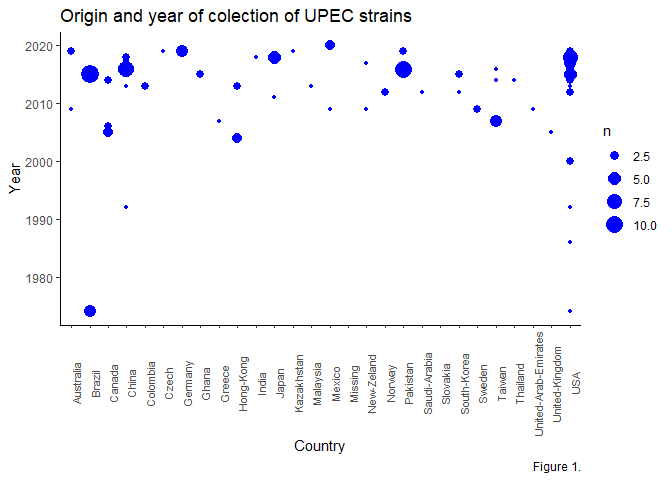
\includegraphics{Report_files/figure-latex/Figure1-1.pdf}

The image showed clearly that we have analysis sequence in the period of
2010 to 2020, the distribution also showed a dominance of USA data, with
Brazil and China whom had little explosions of genomes sequences. Mexico
in particular are a little under represent, and we proudly said that all
the genomes in this chart from Mexico are be from our laboratory.

However, we can also analyse the data using a four variable graphic. In
this case, we only select the two groups that we are more interested.
The Urinary tract Infections (UTI) versus the Recurrent ITU.

\begin{Shaded}
\begin{Highlighting}[]
\CommentTok{\#Use the filter option to make a new table with only RUTI }
\NormalTok{RUTI}\OtherTok{\textless{}{-}}\NormalTok{ database }\SpecialCharTok{\%\textgreater{}\%} \FunctionTok{filter}\NormalTok{(Disease}\SpecialCharTok{==}\StringTok{"RUTI"}\NormalTok{)}
\NormalTok{UTI}\OtherTok{\textless{}{-}}\NormalTok{ database }\SpecialCharTok{\%\textgreater{}\%} \FunctionTok{filter}\NormalTok{(Disease}\SpecialCharTok{==}\StringTok{"UTI"}\NormalTok{)}
\FunctionTok{nrow}\NormalTok{(RUTI)}
\end{Highlighting}
\end{Shaded}

\begin{verbatim}
## [1] 22
\end{verbatim}

\begin{Shaded}
\begin{Highlighting}[]
\FunctionTok{nrow}\NormalTok{(UTI)}
\end{Highlighting}
\end{Shaded}

\begin{verbatim}
## [1] 83
\end{verbatim}

\begin{Shaded}
\begin{Highlighting}[]
\NormalTok{RUTI\_vs\_UTI}\OtherTok{\textless{}{-}}\FunctionTok{rbind}\NormalTok{(RUTI,UTI)}
\FunctionTok{nrow}\NormalTok{(RUTI\_vs\_UTI)}
\end{Highlighting}
\end{Shaded}

\begin{verbatim}
## [1] 105
\end{verbatim}

With this new data we can make a graphic that allow four variables to
compare the UTI vs RUTI strains.

\begin{Shaded}
\begin{Highlighting}[]
\NormalTok{Four\_variables\_graph }\OtherTok{\textless{}{-}} \FunctionTok{ggplot}\NormalTok{ (}\AttributeTok{data =}\NormalTok{ RUTI\_vs\_UTI, }\AttributeTok{mapping =} \FunctionTok{aes}\NormalTok{(}\AttributeTok{y=}\NormalTok{Phylogroup, }\AttributeTok{x=}\NormalTok{Disease, }\AttributeTok{color=}\NormalTok{ Year)) }\SpecialCharTok{+} \FunctionTok{geom\_count}\NormalTok{() }\SpecialCharTok{+} \FunctionTok{labs}\NormalTok{(}\AttributeTok{title =} \StringTok{"UTI versus RUTI"}\NormalTok{, }\AttributeTok{caption =} \StringTok{"Figure 2."}\NormalTok{) }\SpecialCharTok{+} \FunctionTok{facet\_wrap}\NormalTok{(}\StringTok{"MLST"}\NormalTok{)}\SpecialCharTok{+} \FunctionTok{theme\_bw}\NormalTok{() }\SpecialCharTok{+} \FunctionTok{theme}\NormalTok{(}\AttributeTok{axis.text.x =} \FunctionTok{element\_text}\NormalTok{(}\AttributeTok{size=}\DecValTok{8}\NormalTok{, }\AttributeTok{angle=}\DecValTok{90}\NormalTok{))}
\NormalTok{Four\_variables\_graph}
\end{Highlighting}
\end{Shaded}

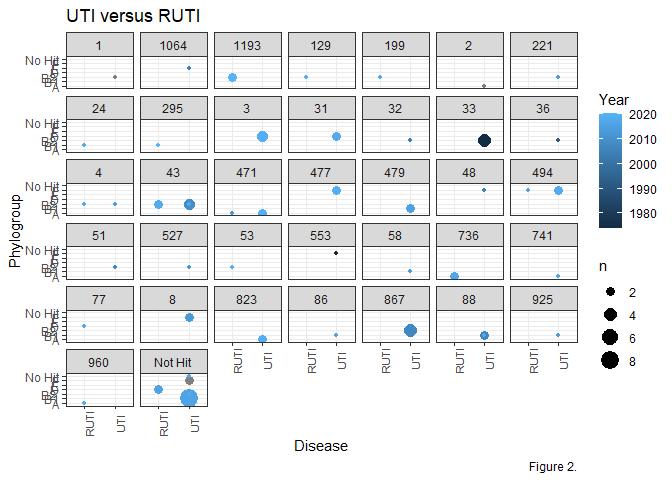
\includegraphics{Report_files/figure-latex/unnamed-chunk-4-1.pdf}

With that information we clearly see that are MLST exclusive for RUTI
and for UTI. In 4, 43, 471, and 494, are for UTI strains, while 1, 1193,
129, 199, 24, 295, 736, and 77 are ST exclusive for RUTI. A brief search
in PubMed, associated 1193 ST with a multidrug resistant bacteria.

Focused in the new information the complete genome and the accessory
sequences was downloading from NCBI. For make the work to find the FimH
sequence more easy, the next script were used.

This was used in the directory ``genomes'', once run the script identify
the 53\% of the sequence, sadly the successes of this script are relate
to the appropriately annotation of the sequences. That is a problem in
our case, because at least the 50\% of the data are no identify.
However, manually finished the database of all the FimH genome, the text
file was called FimH\_pb.txt

\begin{Shaded}
\begin{Highlighting}[]
\NormalTok{fimH\_database }\OtherTok{\textless{}{-}} \FunctionTok{read.delim}\NormalTok{(}\StringTok{"./data/FimH\_pb.txt"}\NormalTok{, }\AttributeTok{header =} \ConstantTok{FALSE}\NormalTok{)}
\FunctionTok{head}\NormalTok{ (fimH\_database)}
\end{Highlighting}
\end{Shaded}

\begin{verbatim}
##                                                                                 V1
## 1                                                                         >00-3076
## 2 ATGAAACGAGTTATTACCCTGTTTGCTGTACTGCTGATGGGCTGGTCGGTAAATGCCTGGTCATTCGCCTGTAAAACCGC
## 3 CAATGGTACAGCTATCCCTATTGGCGGTGGCAGCGCTAATGTTTATGTAAACCTTGCGCCTGCCGTGAATGTGGGGCAAA
## 4 ACCTGGTCGTAGATCTTTCGACGCAAATCTTTTGCCATAACGATTATCCGGAAACCATTACAGACTATGTCACACTGCAA
## 5 CGAGGCTCGGCTTATGGCGGCGTGTTATCTAATTTTTCCGGGACCGTAAAATATAGTGGCAGTAGCTATCCATTTCCGAC
## 6 CACCAGCGAAACGCCGCGGGTTGTTTATAATTCGAGAACGGATAAGCCGTGGCCGGTGGCGCTTTATTTGACGCCTGTGA
\end{verbatim}

This data base was analyse using the Mesquite program, in this scenario
a alignment with Clustal W and tree was performed. The data showed that
the RUTI strains are located around of the UTI. Cleary that the FimH
allele are not related with the RUTI phenotype.

\includegraphics{images/tree-02.jpg}

However, with the Beauti and Beast programs, we develop a Bayesian
analysis, to obtain a likelihood probability, based in RUTI trait.

\begin{Shaded}
\begin{Highlighting}[]
\CommentTok{\#Import data set of Beast. *.log data contain, likelihood, frecuency, position.}
\NormalTok{FimH\_pb.log }\OtherTok{\textless{}{-}} \FunctionTok{read.delim}\NormalTok{(}\StringTok{"\textasciitilde{}/GitHub/FimH\_Variations/data/FimH\_pb.log.txt"}\NormalTok{, }\AttributeTok{comment.char=}\StringTok{"\#"}\NormalTok{)}
\CommentTok{\#With a frecuency graphic we can considerate if there are a posible selection.}
\NormalTok{frecuency}\OtherTok{\textless{}{-}}\FunctionTok{ggplot}\NormalTok{(FimH\_pb.log, }\FunctionTok{aes}\NormalTok{(}\AttributeTok{x=}\NormalTok{frequencies1)) }\SpecialCharTok{+} \FunctionTok{geom\_histogram}\NormalTok{(}\AttributeTok{bins =} \DecValTok{50}\NormalTok{, }\AttributeTok{color =} \StringTok{"black"}\NormalTok{, }\AttributeTok{fill =} \StringTok{"blue"}\NormalTok{) }\SpecialCharTok{+} \FunctionTok{theme\_minimal}\NormalTok{() }\SpecialCharTok{+}\FunctionTok{labs}\NormalTok{(}\AttributeTok{title =} \StringTok{"Histogram of the frecuency of Likelihood"}\NormalTok{, }\AttributeTok{caption =} \StringTok{"Figure 3."}\NormalTok{)}
\NormalTok{frecuency}
\end{Highlighting}
\end{Shaded}

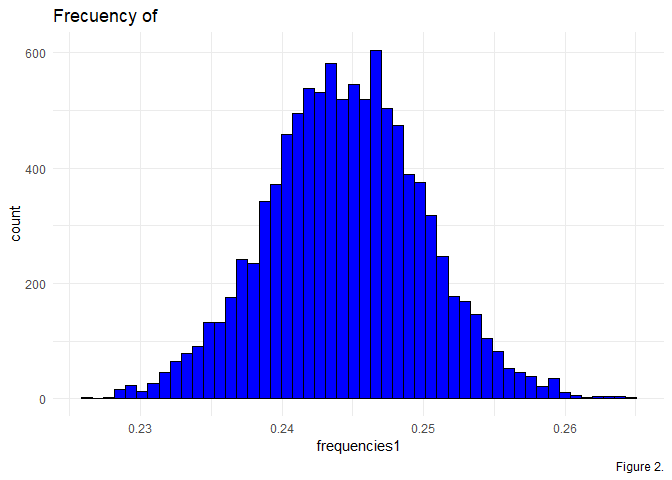
\includegraphics{Report_files/figure-latex/unnamed-chunk-6-1.pdf}

In the graphic of frequency, we can see that the data are centered,
indicative that maybe we don't have a selective presion. Also, the
calculate likelihood it is not significative, because the results are
minor to zero.

\begin{Shaded}
\begin{Highlighting}[]
\NormalTok{neutral}\OtherTok{\textless{}{-}}\FunctionTok{subset}\NormalTok{(FimH\_pb.log,FimH\_pb.log}\SpecialCharTok{$}\NormalTok{likelihood }\SpecialCharTok{\textgreater{}} \DecValTok{0}\NormalTok{)}
\NormalTok{problem}\OtherTok{\textless{}{-}}\FunctionTok{subset}\NormalTok{(FimH\_pb.log,FimH\_pb.log}\SpecialCharTok{$}\NormalTok{treeLikelihood }\SpecialCharTok{\textgreater{}}\DecValTok{0}\NormalTok{)}
\NormalTok{neutral}
\end{Highlighting}
\end{Shaded}

\begin{verbatim}
##  [1] state                joint                prior               
##  [4] likelihood           treeModel.rootHeight age.root.           
##  [7] treeLength           tmrca.RUTI.          age.RUTI.           
## [10] constant.popSize     kappa                frequencies1        
## [13] frequencies2         frequencies3         frequencies4        
## [16] clock.rate           meanRate             treeLikelihood      
## [19] branchRates          coalescent          
## <0 rows> (or 0-length row.names)
\end{verbatim}

\begin{Shaded}
\begin{Highlighting}[]
\NormalTok{problem}
\end{Highlighting}
\end{Shaded}

\begin{verbatim}
##  [1] state                joint                prior               
##  [4] likelihood           treeModel.rootHeight age.root.           
##  [7] treeLength           tmrca.RUTI.          age.RUTI.           
## [10] constant.popSize     kappa                frequencies1        
## [13] frequencies2         frequencies3         frequencies4        
## [16] clock.rate           meanRate             treeLikelihood      
## [19] branchRates          coalescent          
## <0 rows> (or 0-length row.names)
\end{verbatim}

\hypertarget{conclusions}{%
\subsubsection{Conclusions}\label{conclusions}}

There are not signs of adtaptative evolution in fimH gene from a
Bayesian analysis of RUTI versus ITU.

\hypertarget{bibliografuxeda}{%
\subsubsection{Bibliografía:}\label{bibliografuxeda}}

McLay, R. B., \emph{et al.}, (2018). 34(3), 1133-1142.

Tseng, C. C., \emph{et al.}, (2020).

Sokurenko, E. \emph{et al.}, (1998). 95(15), 8922-8926.

Paul, S., \emph{et al.}, (2013). 195(2), 231-242.

Joensen, K. G., \emph{et al.}, (2015). \emph{53}(8), 2410-2426.

\begin{verbatim}
        \       Find your way       /
         \            and          /   
          \    change the world  [|:  
           \    until your last /[|:  [|:
     |:]    \      breath      / [|:  [|:
     |:]   |]\                /  [|:  [|:   :|]
     |:]   |] \   <     >   [  [ [|:  [|:   :|]
    [|:]  :|]  ]   < M >   [  [  [|: [|:   :|]
    [|:   :|]  ]\   < >   /[  [    [ |:   :|]  
    [|:   :|]  ] \   v   /  [. [|:  [|:   |:|]
    [|:   :|] |]  ]      [   [. [|:  [|: :|:|]
    [|:   :|] |]  ]  (#) [   [. [|:  [|: :|]
    [|:|:|:|] |]  / .nHn.\   [. [|:  [|: :|]
        |:|]  |] / HHHHH.\  [. [|:  [|:|:|]
        |:|]  |]/  `HH("N  \ [. [|:  [|:
        |:|]  |]    HHH  "  \[_ [|:  [|:
        :|]  /      NNN      \  [|:  [|:  
        :|] /       N/"       \ [|:  [|:  
        :|]/        N H        \[|:  [|:
        :|]         N           \|:  [|:
         /          q,           \   [|:
        /                         \  [|:
\end{verbatim}

\end{document}
